\documentclass{article}
\usepackage{listings}
\usepackage{color}
\usepackage{amsmath}
\usepackage{amsfonts}
\usepackage{amssymb}
\usepackage{caption}
\usepackage{polski}
\usepackage{indentfirst}
\usepackage{graphicx}
\usepackage{pdfpages}
\usepackage{gauss}
\usepackage[section]{placeins}

\DeclareCaptionType{equ}[][List of equations]
\captionsetup[equ]{labelformat=empty}

%script adding bars in matrix
\usepackage{etoolbox}
\makeatletter
\patchcmd\g@matrix
 {\vbox\bgroup}
 {\vbox\bgroup\normalbaselines}% restore the standard baselineskip
 {}{}
\makeatother

\newcommand{\BAR}{%
  \hspace{-\arraycolsep}%
  \strut\vrule % the `\vrule` is as high and deep as a strut
  \hspace{-\arraycolsep}%
}
\definecolor{dkgreen}{rgb}{0,0.6,0}
\definecolor{gray}{rgb}{0.5,0.5,0.5}
\definecolor{mauve}{rgb}{0.58,0,0.82}

\lstset{frame=tb,
  language=Python,
  aboveskip=3mm,
  belowskip=3mm,
  showstringspaces=false,
  columns=flexible,
  basicstyle={\small\ttfamily},
  numbers=none,
  numberstyle=\tiny\color{gray},
  keywordstyle=\color{blue},
  commentstyle=\color{dkgreen},
  stringstyle=\color{mauve},
  breaklines=true,
  breakatwhitespace=true,
  tabsize=3,
  extendedchars=\true,
  inputencoding=utf8x,
}

\lstset{literate={ą}{{\k{a}}}1 {ł}{{\l{}}}1 {ń}{{\'n}}1 {ę}{{\k{e}}}1 {ś}{{\'s}}1 {ż}{{\.z}}1 {ó}{{\'o}}1 {ź}{{\'z}}1 {Ą}{{\k{A}}}1 {Ł}{{\L{}}}1 {Ń}{{\'N}}1 {Ę}{{\k{E}}}1 {Ś}{{\'S}}1 {Ż}{{\.Z}}1 {Ó}{{\'O}}1 {Ź}{{\'Z}}1 }

\begin{document}
\title{Sprawozdanie nr. 2 - Metody numeryczne i optymailzacja}
\author{Jakub Andryszczak 259519,\\ Jakub Żak 244255,\\ Maciej Cierpisz 249163}
\date{}
\maketitle

\newpage
\tableofcontents
%Tutaj zaczyna się wstęp

\newpage
\section{Zadanie nr. 1}
Wyznacz ręcznie pary własne (wyniki potwierdź obliczeniami komputerowymi):
\begin{equation}
  A_{1} =
  \begin{gmatrix}[b]
    21 & -6 & 0 \\
    -6 & 18 & 6 \\
    0 & 6 & 15
\end{gmatrix}
,
A_{2}=
\begin{gmatrix}[b]
  0 & -2 & 1\\
  1 & 3 & -1 \\
  0 & 0 & 1
\end{gmatrix}
,
A_{3}=
\begin{gmatrix}[b]
  5 & 4 & 2 & 1 \\
  0 & 1 & -1 & -1 \\
  -1 & -1 & 3 & 0 \\
  1 & 1 & -1 & 2
\end{gmatrix}
\end{equation}
Sprawdź czy ślad macierzy jest równy sumie jej wartości własnych. Które macierze są diagonalizowalne i dlaczego? Czy któraś z tych macierzy jest osobliwa?

Macierzą osobliwą nazywamy taką, której wyznacznik jest równy zero. Dla każdej z wcześniej wymienionych macierzy wyliczono ich wyznaczniki.
\begin{equation}
  A_{1}= 21*18*15 + 6*(-6)*0 + 0*6*(-6) - (21*6 * 6) - (-6* -6 * 15) - (0 * 0 * 18) = 4374
\end{equation}
Wynik wyznacznika dla pierwszej macierzy nie jest równy zeru, a zatem wartość $A_{1}$ nie należy do macierzy osobliwych.
\begin{equation}
  A_{2}=2
\end{equation}
\begin{equation}
  A_{3}=32
\end{equation}
Z obliczeń wynika żadna z macierzy nie spełnia warunku osobliwości.

Następnie obliczono ślad powyższych macierzy. Ślad macierzy jest to suma elementów leżących na przekątnej danej macierzy. A zatem:
\begin{equation}
  A_{1}=54
\end{equation}
\begin{equation}
  A_{2}=4
\end{equation}
\begin{equation}
  A_{3}=11
\end{equation}

Do wyznaczenia par i wartości własnych macierzy oraz sprawdzenia czy podane macierze są diagonalizowalne obliczono wyznacznik $det(A-\lambda I)=0$:
\begin{equation}
  det(A_{1}-\lambda)=(21-\lambda)(18-\lambda)(15-\lambda) - (21-\lambda)*6*6 -(15-\lambda)*-6*-6= 0
\end{equation}
\begin{equation}
  \lambda^{3} - 54\lambda^{2} + 891\lambda - 4374 = 0
\end{equation}
Znaleziono pierwsze miejsce zerowe równania równe 18. Po podzieleniu wielomian wygląda następująco:
\begin{equation}
  x^2 - 36x + 243 = 0
\end{equation}
Po wyliczeniu delty wyznaczono wartości własne tego równania: $\lambda_1 = 9$, $\lambda_2 = 18$, $\lambda_3 =27$.
Podstawiajając pod macierz $A_1$ wartość $\lambda_1$ otrzymujemy układ równań:
\begin{equation}
  \begin{gmatrix}[b]
   12 & -6 & 0\\
   -6 & 9 & 6\\
   0 & 6 & 6
  \end{gmatrix}
  \begin{gmatrix}[b]
    x\\y\\z
  \end{gmatrix}
  =
  \begin{gmatrix}[b]
    0\\0\\0
  \end{gmatrix}
\end{equation}
Obliczamy w ten sposób wektor własny którego wartość jest równa:
\begin{equation}
  \begin{gmatrix}[b]
   -2\\2\\1 
  \end{gmatrix}
\end{equation}
Dla $\lambda_2$ i $\lambda_3$ wektory własne prezentują się następująco:
\begin{equation}
  \lambda_2 =
  \begin{gmatrix}[b]
    2\\1\\2
  \end{gmatrix}
  ,
  \lambda_3 = 
  \begin{gmatrix}[b]
    -1\\-2\\2
  \end{gmatrix}
\end{equation}
Tym samym powstaje nam macierz
\begin{equation}
  P = 
  \begin{gmatrix}[b]
    1 & 2 & -2 \\
    -2 & 1 & 2 \\
    2 & 2 & 1
  \end{gmatrix}
\end{equation}
A macierzą odwrotną będzie macierz
\begin{equation}
  P^{-1} =
  \begin{gmatrix}[b]
    -\frac{1}{9}&-\frac{2}{9}&\frac{2}{9}\\
    \frac{2}{9}&\frac{1}{9}&\frac{2}{9}\\
    -\frac{2}{9}&\frac{2}{9}&\frac{1}{9}
  \end{gmatrix}
\end{equation}
Aby sprawdzić czy dana macierz jest diagonalizowalną należy sprawdzić czy A` jest równa macierzy A.
\begin{equation}
  \begin{gmatrix}[b]
    1 & 2 & -2 \\
    -2 & 1 & 2 \\
    2 & 2 & 1
  \end{gmatrix}
  *
  \begin{gmatrix}[b]
    -\frac{1}{9}&-\frac{2}{9}&\frac{2}{9}\\
    \frac{2}{9}&\frac{1}{9}&\frac{2}{9}\\
    -\frac{2}{9}&\frac{2}{9}&\frac{1}{9}
  \end{gmatrix}
  *
  \begin{gmatrix}[b]
    9 & 0 & 0\\
    0 & 18 & 0\\
    0 & 0 & 27
  \end{gmatrix}
  =
  \begin{gmatrix}[b]
    21 & -6 & 0 \\
    -6 & 18 & 6 \\
    0 & 6 & 15
  \end{gmatrix}
\end{equation}
A zatem macierz jest diagonalizowalna i nieosobliwa, a ślad macierzy jest równy sumie wartości własnych

Dla przykładu drugiego równanie prezentują się następująco:
\begin{equation}
  det(A_2 -\lambda) =-\lambda^{3} + 4\lambda^{2}-5\lambda + 2 = 0
\end{equation}
\begin{equation}
  \lambda^3-4\lambda^2+5\lambda -2 = 0
\end{equation}
Suma współczynników jest równa 0, a zatem $\lambda_1$=1. Kolejno podzielono wielomian przez ($\lambda-1$).
\begin{equation}
  \lambda^2 - 3\lambda + 2 = 0
\end{equation}
Następnie wyliczono $\Delta$ ze wzoru $\Delta = b^2 - 4ac$, której wartość wyszła 1. Ze względu na to obliczono pierwiastki za pomocą wzoru:
\begin{equation}
  x=\frac{-b \pm \sqrt[]{\Delta}}{2a} = \frac{3 \pm \sqrt[]{1}}{2}
\end{equation}
Wynikami tego działania są $\lambda_2 = 1$ i $\lambda_3 = 2$.
Dla wartości $\lambda_1$,$\lambda_2$ i $\lambda_3$ wyliczono wektory własne.
\begin{equation}
  \lambda_1 = 
  \begin{gmatrix}[b]
    -1\\1\\0
  \end{gmatrix}
  , \lambda_2 =
  \begin{gmatrix}[b]
    1\\0\\1
  \end{gmatrix}
  , \lambda_3 =
  \begin{gmatrix}[b]
    -2\\1\\0
  \end{gmatrix}
\end{equation}
Tak jak w przykładzie wyżej do sprawdzenia czy macierz jest diagonalizowalna obliczono:
\begin{equation}
  \begin{gmatrix}[b]
   1&-2&-1\\
   0&1&1\\
   1&0&0 
  \end{gmatrix}
  *
  \begin{gmatrix}[b]
    1&0&0\\
    0&1&0\\
    0&0&2
  \end{gmatrix}
  *
  \begin{gmatrix}[b]
    0&0&1\\
    -1&-1&1\\
    1&2&-1
  \end{gmatrix}
  =
  \begin{gmatrix}[b]
    0 & -2 & 1\\
    1 & 3 & -1 \\
    0 & 0 & 1
  \end{gmatrix}
\end{equation}
Macierz jest diagonalizowalna i nieosobliwa, a ślad macierzy jest równy sumie wartości własnych.
Trzeci przykład:
\begin{equation}
  det(A_3 -\lambda) =\lambda^{4}-11\lambda^{3} + 42\lambda^{2}-64\lambda + 32 = 0
\end{equation}
Znaleziono wartości własne równe 1 i 2. Po podzieleniu wielomianu przez ($\lambda-1$) i ($\lambda -2$) otrzymujemy $\lambda^2 -8\lambda+16$. Ostatnią wartością własną jest $\lambda=4$. 
Wyliczając wektory własne $\lambda_3$ ma tą samą wartość co $\lambda_4$ a zatem macierz nie może być diagonalizowalna ze względu na powtarzające się wektory własne. Jest ona również nieosobliwa, a ślad jest równy sumie wartości własnych.
\newpage

\section{Zadanie nr. 2}

Wyznacz największą i najmniejszą wartość własną stosując metodę Powera zwykłą
i z przesunięciem:
\begin{equation}
  A = 
  \begin{gmatrix}[b]
    4&2&0&0\\
    1&4&1&0\\
    0&1&4&1\\
    0&0&2&4
  \end{gmatrix}
\end{equation}
Napisano algorytm wyznaczający największą i najmniejszą wartość własną:
\begin{lstlisting}

    import numpy as np

    A = np.array([ [4, 2, 0, 0],
                  [1, 4, 1, 0],
                  [0, 1, 4, 1],
                  [0, 0, 2, 4],])
    
    x = np.random.rand(4)
    print(x)
    print()
    
    def normal_power_method(A,x):
        for i in range(200):
         x = np.dot(A,x)
         x  = x/np.linalg.norm(x)
        
        return np.dot(np.dot(A,x),x)/np.dot(x, x)
    
    def shifted_power_method(A, x0, tol=1e-6):
      n = len(A)
      # Estimate a shift close to the smallest eigenvalue
      sigma = np.trace(A) / n
      x = x0.copy()
      for _ in range(200):
        y = np.dot(A, x) - sigma * x
    
      lambda_ = np.dot(x.T, np.dot(A, x))
      return lambda_
       
    
    lambda1 = normal_power_method(A, x) 
    lambda2 = 1 / normal_power_method(A, x)
    lambda3 = shifted_power_method(A, x)
    lambda4 = 1 / shifted_power_method(A, x)
    
    print("Largrest eigenvalue normal power",lambda1)
    print("Smallest eigenvalue normal power", lambda2)
    print("Largest eigenvalue shifted power", lambda3)
    print("Smallest eigenvalue shifted power", lambda4)
  
  \end{lstlisting}
  Poniżej wynik działania programu:
  \begin{figure}[h]
    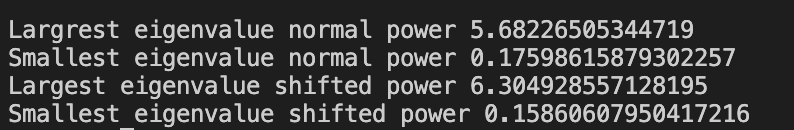
\includegraphics[scale=0.7]{image.png}
    \centering
    \caption*{Rys. 1 Wyniki obliczeń}
    \end{figure}

\section{Zadanie nr. 3}
Rozwiąż układ równań różniczkowych zwyzczajnych:
\begin{center}
  $
  \frac{du}{dt} = Pu $ dla $u_{0}=
  \begin{gmatrix}[b]
    8\\5
  \end{gmatrix}$
  oraz P=$
  \begin{gmatrix}[b]
    4&-5\\2&-3
  \end{gmatrix}
$
\end{center}

Układy równań wygląda następująco:
\begin{equation}
 \frac{du_{1}}{dt} = 4u_{1}-5u_{2}
\end{equation}
\begin{equation}
  \frac{du_{2}}{dt} = 2u_{1}-5u_{2}
 \end{equation}
 
 Równanie $\frac{du}{dt} = lambda u$ można przekształcić na $ u = \alpha e^{\lambda t}$, a następnie podstawiajając uzyskujemy:
 \begin{equation}
  \alpha_{1}\lambda e^{\lambda t} = 4 \alpha_{1}e^{\lambda t} -5\alpha_{2}e^{\lambda t}
 \end{equation}
 \begin{equation}
  \alpha_{2}\lambda e^{\lambda t} = 2 \alpha_{1}e^{\lambda t} -3\alpha_{2}e^{\lambda t}
 \end{equation} 
 Ze układu obustronnie usuwamy $e^{\lambda t}$ a pozostałe wartości zapisujemy w macierzach:
 \begin{equation}
  \begin{gmatrix}[b]
    4 & -5\\
    2 & -3
  \end{gmatrix}
  \begin{gmatrix}[b]
    \alpha_1\\
    \alpha_2
  \end{gmatrix}
  =\lambda
  \begin{gmatrix}[b]
    \alpha_1\\
    \alpha_2
  \end{gmatrix}
 \end{equation}
 Następnie jak w zadaniu pierwszym przystąpiono do wyliczenia $det(A \lambda I)$
 \begin{equation}
  det
  \begin{gmatrix}
    4-\lambda & -5 \\
    2 & -3-\lambda
  \end{gmatrix}
  =(4-\lambda)(-3-\lambda)+10 = \lambda^{2}-\lambda-2 = 0
 \end{equation}
 Wyliczono, że wartościami własnymi są $\lambda_1 =-1$ i  $\lambda_2 =2$.
 
 Podstawiajając wartości własne wyliczamy wektory własne.
 Dla $\lambda_1 = -1$:
 \begin{equation}
  \begin{gmatrix}[b]
    5 & -5 \\
    2 & -2
  \end{gmatrix}
  x_{1} = 0
  \Rightarrow
  x_{1}=
  \begin{gmatrix}[b]
    1\\1
  \end{gmatrix}
 \end{equation}
 Dla $\lambda_2 = 2$:
 \begin{equation}
  \begin{gmatrix}[b]
    2 & -5 \\
    2 & -5
  \end{gmatrix}
  x_{2} = 0
  \Rightarrow
  x_{2}=
  \begin{gmatrix}[b]
    5\\2
  \end{gmatrix}
 \end{equation}
 Rozwiązanie tego zadania wygląda następująco:
 \begin{center}
  $u =c_{1} e^{\lambda_1 t}x_{1} + c_{2}e^{\lambda_{2}t}x_{2}$
 \end{center}
 Podstawiając $u^{(0)}$ wyliczamy wartości $C_1$ i $C_2$:
 \begin{equation}
  c_{1}x_{1} + c_{2}x_{2} = u^{(0)}, \Rightarrow
  \begin{gmatrix}[b]
    1 & 5\\
    1 & 2
  \end{gmatrix}
  \begin{gmatrix}[b]
    c_1\\c_2
  \end{gmatrix}
  =
  \begin{gmatrix}[b]
    8 \\ 5
  \end{gmatrix}
  \Rightarrow
  \begin{gmatrix}[b]
    c_1\\c_2
  \end{gmatrix}
  =
  \begin{gmatrix}[b]
    3\\1
  \end{gmatrix}
 \end{equation}
 Odpowiedzią dla tego zadania jest funkcja:
 \begin{equation}
  u = 3 e^{-t}
  \begin{gmatrix}[b]
    1\\1
  \end{gmatrix}
  + e^{2t}
  \begin{gmatrix}[b]
    5\\2
  \end{gmatrix}
 \end{equation}
\section{Zadanie nr. 4}
Wyznacz $A^{100}$ metodą diagonalizacji macierzy 
\begin{equation}
  A =
  \begin{gmatrix}[b]
  4&3\\1&2
\end{gmatrix}
\end{equation}


Obliczanie wartości własnych:
\begin{equation}
  \det(A - tI) = \begin{bmatrix} 4-t & 3 \\ 1 & 2-t \end{bmatrix} = t^2 - 6t + 5 = (t-1)(t-5) =0 
\end{equation}

\begin{equation}
\begin{cases}
  t_1 = 1\\
  t_2 = 5
\end{cases}
\end{equation}\\

Obliczanie wektorów własnych:\\
\begin{equation}
  (A - t_{1}I) = \begin{bmatrix} 3 & 3 \\ 1 & 1 \end{bmatrix}
\end{equation}

\begin{equation}
  (A - tI)*v = 0
\end{equation}\\

\[
  \centering
  \linespread{2}\selectfont
  \addtolength{\arraycolsep}{10pt}
 \begin{gmatrix}[b]
3 & 3 & \BAR & 0\\
1 & 1 & \BAR & 0
\rowops
\mult{0}{\cdot \left(\frac1{3}\right)}
\add[-1]01
 \end{gmatrix}
\]

\[
  \centering
  \linespread{2}\selectfont
  \addtolength{\arraycolsep}{10pt}
 \begin{gmatrix}[b]
1 & 1 & \BAR & 0\\
0 & 0 & \BAR & 0
 \end{gmatrix}
\]

\begin{equation}
  X = \begin{bmatrix} -1  \\ 1  \end{bmatrix}
\end{equation}

\begin{equation}
  (A - t_{1}I) = \begin{bmatrix} -1 & 3 \\ 1 & -3 \end{bmatrix}
\end{equation}

\begin{equation}
  (A - tI)*v = 0
\end{equation}\\

\[
  \centering
  \linespread{2}\selectfont
  \addtolength{\arraycolsep}{10pt}
 \begin{gmatrix}[b]
3 & 3 & \BAR & 0\\
1 & 1 & \BAR & 0
\rowops
\mult{0}{\cdot \left( -1 \right)}
\add[-1]01
 \end{gmatrix}
\]

\[
  \centering
  \linespread{2}\selectfont
  \addtolength{\arraycolsep}{10pt}
 \begin{gmatrix}[b]
1 & -3 & \BAR & 0\\
0 & 0 & \BAR & 0
 \end{gmatrix}
\]

\begin{equation}
  X = \begin{bmatrix} 3  \\[6pt] 1  \end{bmatrix}
\end{equation}

Obliczanie potęgi macierzy po diagonalizacji:

\begin{equation}
  D = \begin{bmatrix} 1 & 0  \\[6pt] 0 & 5  \end{bmatrix}
\end{equation}

\begin{equation}
  P = \begin{bmatrix} -1 & 3  \\[6pt] 1 & 1  \end{bmatrix}
\end{equation}

\begin{equation} 
  P^{-1} = \begin{bmatrix} -\frac{1}{4} & \frac3{4}  \\[6pt]
    \frac{1}{4} & \frac{1}{4}  \end{bmatrix}
\end{equation}

\begin{equation} 
  A^{100} = P*D^{100}*P^{-1}
\end{equation}

\begin{equation} 
  A^{100} = \begin{bmatrix} -1 & 3  \\[6pt] 1 & 1  \end{bmatrix} * \begin{bmatrix} 1^{100} & 0  \\[6pt] 0 & 5^{100}  \end{bmatrix} * \begin{bmatrix} -\frac{1}{4} & \frac3{4}  \\[6pt]
    \frac{1}{4} & \frac{1}{4}  \end{bmatrix}
\end{equation}


\section{Zadanie nr. 5}
Wykreśl dyski Gershgorina i określ lokalizację wwartości własnych macierzy:
\begin{equation}
  A_1 =
  \begin{gmatrix}[b]
    -2 & -1 & 0\\
    2 & 0 & 0\\
    0 & 0 & 2
  \end{gmatrix}
  ,
  A_2 = 
  \begin{gmatrix}[b]
    5 & 1 & 1\\
    0 & 6 & 1\\
    0 & 0 & -5
  \end{gmatrix}
  ,
  A_3 =
  \begin{gmatrix}[b]
    5.2 & 0.6 & 2.2\\
    0.6 & 6.4 & 0.5\\
    2.2 & 0.5 & 4.7
  \end{gmatrix},
\end{equation}
Zaznacz na dyskach lokalizację dokładnych wartości własnych wyznaczonych dowolną metodą.

\begin{lstlisting}
  import numpy as np
  import matplotlib.pyplot as plt
  
  def gershgorin_circles(matrix):
      """
      Generuje środki i promienie dysków Gershgorina dla danej macierzy.
      """
      n = matrix.shape[0]
      centers = np.diag(matrix)
      radii = np.sum(np.abs(matrix), axis=1) - np.abs(centers)
      return centers, radii
  
  def plot_gershgorin_circles(matrix, name):
      centers, radii = gershgorin_circles(matrix)
      fig, ax = plt.subplots()
  
      # Rysowanie dysków Gershgorina
      for center, radius in zip(centers, radii):
          circle = plt.Circle((center.real, center.imag), radius, color='blue', fill=False)
          ax.add_artist(circle)
  
      # Obliczanie i rysowanie wartości własnych
      eigenvalues = np.linalg.eigvals(matrix)
      for eigenvalue in eigenvalues:
          plt.scatter(eigenvalue.real, eigenvalue.imag, color='red')
          # Wstawienie wartości własnych jako tekst na wykresie
          plt.text(eigenvalue.real, eigenvalue.imag, f'{eigenvalue:.2f}', fontsize=9, verticalalignment='bottom',horizontalalignment='right')
  
      # Dodanie etykiet dla dokładnych wartości własnych
      for i, (eigenvalue_real, eigenvalue_imag) in enumerate(zip(eigenvalues.real, eigenvalues.imag)):
          ax.annotate(f'lambda{i + 1}', (eigenvalue_real, eigenvalue_imag), textcoords="offset points", xytext=(-10, 10), ha='center')
  
      # Ustawienia wykresu
      ax.set_aspect('equal', 'box')
      plt.grid(True)
      plt.xlabel('Re')
      plt.ylabel('Im')
      plt.title('Dyski Gershgorina i wartości własne macierzy dla macierzy: '+str(name))
      plt.legend()
  
      # Ustaw zakres osi tak, aby pasował do dysków
      x_min = min(centers.real - radii)
      x_max = max(centers.real + radii)
      y_min = min(centers.imag - radii)
      y_max = max(centers.imag + radii)
      ax.set_xlim(x_min - 1, x_max + 1)
      ax.set_ylim(y_min - 1, y_max + 1)
  
      plt.show()
      
  # Przykładowa macierz
  A = np.array([[-2, 1, 0],[2, 0, 0],[0, 0, 2]])
  B = np.array([[5, 1, 1],[0, 6, 1],[0, 0, -5]])
  C = np.array([[5.2, 0.6, 2.2],[0.6, 6.4, 0.5],[2.2, 0.5, 4.7]])
  
  plot_gershgorin_circles(A, "A")
  plot_gershgorin_circles(B, "B")
  plot_gershgorin_circles(C, "C")

\end{lstlisting}
Poniżej wyniki w postaci wykresów:
\begin{figure}[!h]
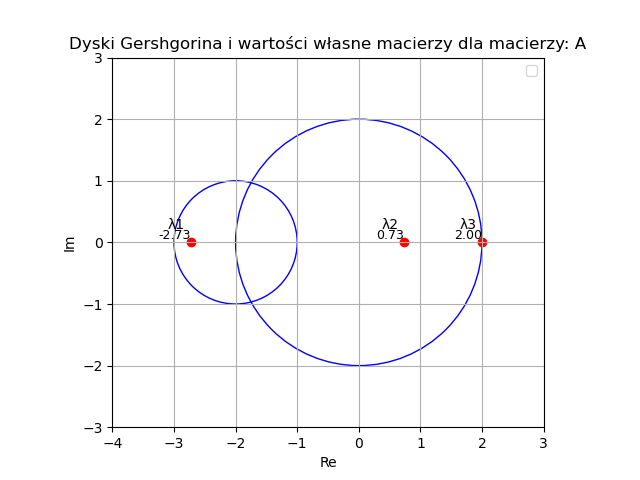
\includegraphics[scale=0.5]{matrixA.png}
\centering
\caption*{Rys. 2 Wyniki macierz A}
\end{figure}

\begin{figure}[!h]
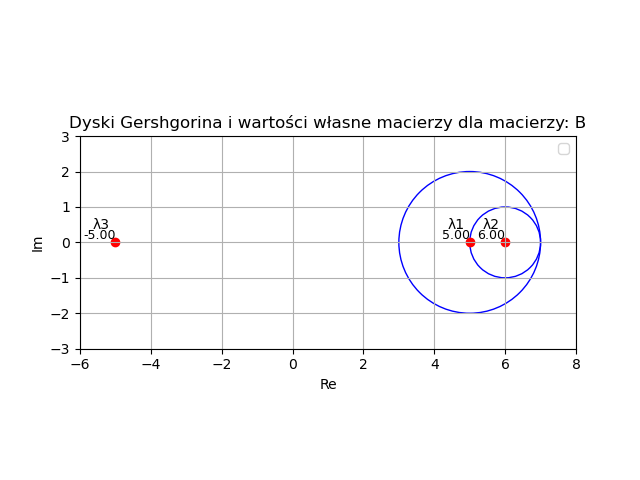
\includegraphics[scale=0.5]{matrixB.png}
\centering
\caption*{Rys. 2 Wyniki macierz B}
\end{figure}

\begin{figure}[!h]
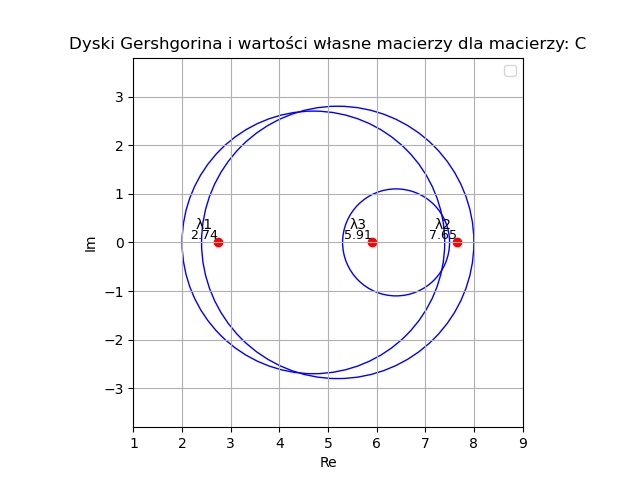
\includegraphics[scale=0.5]{matrixC.png}
\centering
\caption*{Rys. 2 Wyniki macierz C}
\end{figure}

\newpage

\section{Zadanie nr. 6}
Wyznacz rozkład VD macierzy (bez użycia funkcji "svd"):
\begin{equation}
  (a) A_1 = 
  \begin{gmatrix}[b]
    1&1\\
    0&1\\
    1&0
  \end{gmatrix}
  , (b) A_2=
  \begin{gmatrix}[b]
    -1 & 2 & 2
  \end{gmatrix}
  , (c) A_3=
  \begin{gmatrix}[b]
    2&2&2&2\\
    \frac{17}{10}&\frac{1}{10}&-\frac{17}{10}&-\frac{1}{10}\\
    \frac{3}{5}&\frac{9}{5}&-\frac{3}{5}&-\frac{9}{5}
  \end{gmatrix}
\end{equation}
Wyniki obliczeń porównaj z obliczeniami komputerowymi wykorzystującymi funkcję "svd".
\section{Zadanie nr. 7}
Przekształć dowolny obraz (z Internetu) do macierzy o wymiarach 640 x 400 (standard
VGA), a następnie przeskaluj wartości elementów aby: $0\leq x\leq 1$; gdzie x = 0 odpowiada
poziomowi czerni, x = 1 to poziom bieli. Wyznacz SVD takiej macierzy wykorzystując dowolną
implementację algorytmu SVD. Następnie utwórz obraz z faktorów dla następujących przypadków: 10; 20 oraz 40 wartości osobliwych i odpowiadającym im wektorów osobliwych.
\begin{lstlisting}
link = 'https://www.alleycat.org/wp-content/uploads/2019/03/FELV-cat.jpg';
zdjecie = imread(link);

zdjecie_rozmiar = imresize(zdjecie, [640, 400]);

zdjecie_skala = double(zdjecie_rozmiar) / 255;

[U, S, V] = svd(zdjecie_skala);

wart_os = [10, 20, 40];

for w = wart_os
    zdjecie_wart = U(:, 1:w) * S(1:w, 1:w) * V(:, 1:w)';
    zdjecie_wart = max(min(zdjecie_wart, 1), 0);
    imshow(zdjecie_wart);
    pause;
end

\end{lstlisting}  
\end{document} 
